\documentclass[main]{subfiles} 
\graphicspath{{img/}}


\begin{document}

\section{Methodology}
A big difference between real estate and other publicly traded assets is that there is no centralized platform where offers can be tracked. 
In the case of asset classes such as bonds and equity this service is provided by multiple sources such as Bloomberg, Refinitiv and Morningstar.
Historical prices, key financial data, plots and proxies are all available on one single platform.
Something similar is missing for the Swiss real estate market. 

Usually real estate on the various websites is presented as a list of single "tiles",
along with a brief overview of the key data and pictures of the corresponding property (for reference see figure \ref{fig:listing}).
Whilst this is already a solid foundation, 
there is no possibility to see the average cost per square meter in the ZIP code and no real way to compare similar estates.

Given that the data is neither available via an \acs*{api} nor through an already established database,
the decision was made to write an algorithm that scrapes the required data from a website.

\subsection{Choice of Website}

Whilst there exist numerous websites that act as middlemen between buyer and seller such as \verb|www.immoscout24.ch| and \verb|www.homegate.ch|,
all of them suffer from the same underlying problem mentioned in the introduction. 
Selecting and pricing real estate by clicking through every listing is cumbersome and inefficient.
Furthermore, with the data being split up over many websites, 
a buyer might not find his ideal new property, simply by searching on the wrong platform.

An attempt at creating a more transparent and efficient real estate market was made by Comparis. 
On their website, listings from many sources are aggregated and displayed according to their key characteristics.
However, also \verb|www.comparis.ch| does not offer tools for further analysis and does not readily display historical data,
except for increases or decreases in the price in percentage.

For the purpose of creating a database which provides a user with information on as many properties in a given area as possible, 
\verb|www.comparis.ch| is the ideal target for scraping data.


\subsection{Web Scraping}

When creating a web scraping application in python, there are a number of packages and tools to choose from.
These modules include, but are not limited to \pkg[requests], \pkg[BeautifulSoup], \pkg[Scrapy] and last but not least, \pkg[Selenium].
Each come with their advantages and disadvantages. 
The former two modules, \pkg[requests] and \pkg[BeautifulSoup] both come with the bonus of ease of use.
The latter two modules offer more functionality, but have a steeper learning curve.

After several attempts, the choice boiled down to a combination of \pkg[Selenium] and \pkg[Scrapy].
This decision was based on the need to not only collect data on the "top level" of the listing (see \ref{fig:listing}), 
but also the information on the detail page of every single \acs*{url}.

\begin{figure}[htbp]
    \centerline{
        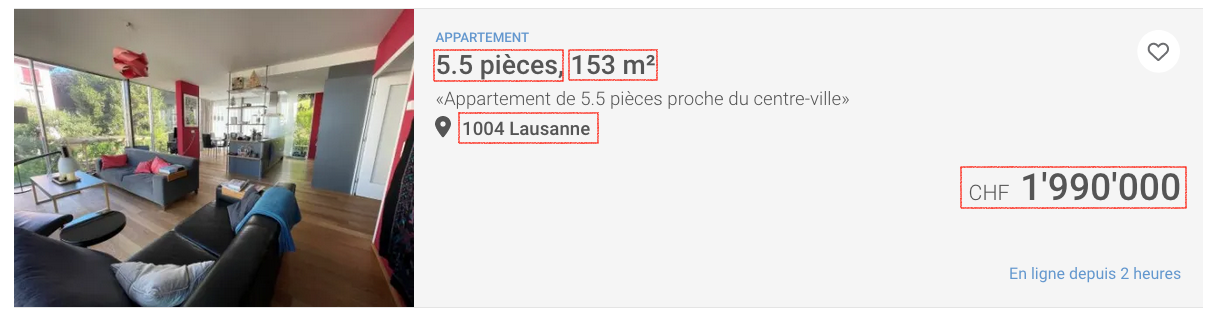
\includegraphics[width = 92mm]{prog_1.png}}
    \caption{Typical Listing on Comparis}
    \label{fig:listing}
\end{figure}

The need for more data was not the only factor that led to this choice.
Today's websites are populated with \js's that procedurally generate the content a user can see.
The \js's may load further information based on simple actions such as scrolling on the page,
clicking a button, or by more complex actions such as hovering over a certain area or logging in somewhere.
For a web scraping service that relies on parsing \acs*{html} (such as \pkg[requests] and \pkg[BeautifulSoup]), 
this poses a major issue.
The way \pkg[requests] works is that it sends a GET request to the website and subsequently returns the source code (\acs*{html}) for further analysis.
However, simply sending a request is not enough to trigger a \js since it needs interaction from the user to generate the content and thus, 
"add" source code.
The source code returned by \pkg[requests] for \js heavy websites generally offers very limited insights.
A common workaround is the scraping the "hidden API" \hly[cite].
Said "hidden API" consists of a \acs*{json} file which, in certain cases contains all the information the \js would generate based on the user action.
Since this  \acs*{json} has its own \acs*{url}, \pkg[requests] can get the data from there, 
and therefore effectively get around the "\js barrier".
Due to the structure of Comparis' website, this was not an option.

\subsection{Scrapy}
Of the largest web scrapers available for python, 
\pkg[Scrapy] usually serves the needs of larger scale web scraping projects.
\pkg[Scrapy]'s main feature is the so-called spider which can be customized to serve many needs.
A spider is set up by using the \pkg[scrapy genspider <example> <example.com>] command 
(after running the \pkg[scrapy startproject] command in the terminal).
Along with the project- and spider folders, scrapy generates several \pkg[.py] 
files that allow granular customization of the spider.
To use a spider, the user has to define a spider class (which inherits all attributes from the class \pkg[scrapy.Spider]),
that tells \pkg[Scrapy] how and in what sequence to scrape which content of a given website.

Websites are created with the user experience in mind first.
This entails that the output of a scraping activity can be very disorganized and filled with unwanted \acs*{html} tags.
Here \pkg[Scrapy] offers a very attractive solution, namely the \pkg[ItemLoader], 
which is defined as a class in the \pkg[items.py] file.
Whilst \pkg[ItemLoader] certainly adds to the steepness of the learning curve, it is a worthwhile endeavor, 
since the scraped data will come out clean already. 
\pkg[ItemLoader] "cleans" the data when it comes in, stores it while the spider is running, 
and generates an output based on the user's preference.

\pkg[Scrapy] can send many requests to a website at once, 
thus speeding up the data gathering process tremendously.
However, even when using all the request headers that a normal browser sends to a website, 
the \pkg[Scrapy] spider's were constantly \acs*{ip}-blocked.

\begin{figure}[htbp]
    \centerline{
        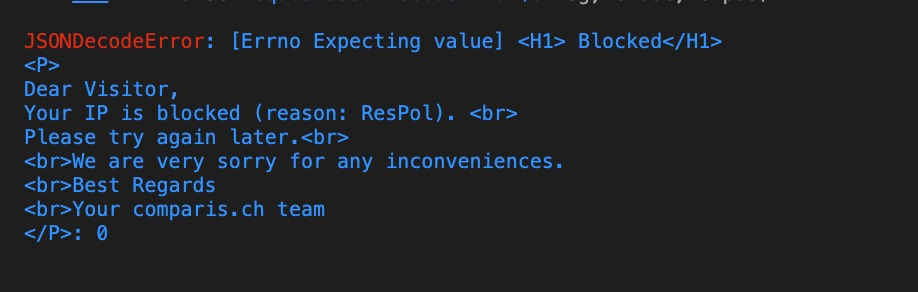
\includegraphics[width = 80mm]{prog_2.png}}
    \caption{IP block when running the spiders}
    \label{fig:block}
\end{figure}

\subsection{Selenium}
Whilst \pkg[Scrapy] works well with extracting data from the website's source code (especially using \acsp*{xpath}'s), 
it is still not possible to navigate \js heavy websites and trigger the scripts that give access to the important information in the source code.
Furthermore, even with the implementation of rotating proxies in scrapy, the \acs*{ip}-block could not be circumvented.

This is where \pkg[Selenium] comes in: \pkg[Selenium] allows a user to control any browser environment,
provided the corresponding driver has been installed.
Controlling a browser offers several advantages, the primary advantage being that the request comes from an actual browser,
which means it will very rarely get blocked. 
The downside is that by sending the requests through a browser window, 
the amount of requests per time is practically reduced to one.
This increases the runtime of the program drastically, 
however it adds the upside that the data collection is successful.

For this project it was decided that by combining \pkg[Selenium] with \pkg[Scrapy], the best of both worlds can be obtained:
reliable data gathering on the one hand, and clean data extraction on the other hand.


\subsection{User platform}
To make the dataset scrapped from Comparis more user-friendly we decided to build a \ac{gui}.
This way the user will be able to search for a property within a certain price range, zip code or with specific features, 
instead or having to go through the full scrapped dataset.
We used the open source library \pkg[tkinter] to model the GUI. We chose this library as it is pre-installed in python.
Moreover it is stable and flexible and provides simple syntax.
\pkg[tkinter] is the perfect tool for this first prototype. However, if the project grows \pkg[tkinter] will not be powerful enough,
therefore we recommend switching to PyQT another \ac{gui} or even REACT for a more professional look. 


\subsection{Structure}
\end{document}